% !TEX TS-program = XeLaTeX
% use the following command:
% all document files must be coded in UTF-8
\documentclass[spanish]{textolivre}
% build HTML with: make4ht -e build.lua -c textolivre.cfg -x -u article "fn-in,svg,pic-align"

\journalname{Texto Livre}
\thevolume{16}
%\thenumber{1} % old template
\theyear{2023}
\receiveddate{\DTMdisplaydate{2023}{6}{25}{-1}} % YYYY MM DD
\accepteddate{\DTMdisplaydate{2023}{7}{13}{-1}}
\publisheddate{\DTMdisplaydate{2023}{9}{4}{-1}}
\corrauthor{Fabiola Sáez-Delgado}
\articledoi{10.1590/1983-3652.2023.46636}
%\articleid{NNNN} % if the article ID is not the last 5 numbers of its DOI, provide it using \articleid{} commmand 
% list of available sesscions in the journal: articles, dossier, reports, essays, reviews, interviews, editorial
\articlesessionname{articles}
\runningauthor{Sáez-Delgado et al.} 
%\editorname{Leonardo Araújo} % old template
\sectioneditorname{Hugo Heredia Ponce}
\layouteditorname{Thaís Coutinho}

\title{Efectividad de las intervenciones con tecnologías para promover la autorregulación del aprendizaje en estudiantes universitarios: un metaanálisis}
\othertitle{Eficácia das intervenções baseadas em tecnologia para promover a aprendizagem autorregulada em estudantes universitários: uma meta-análise}
\othertitle{Effectiveness of technology interventions to promote self-regulation of learning: a meta-analysis}
% if there is a third language title, add here:
%\othertitle{Artikelvorlage zur Einreichung beim Texto Livre Journal}

\author[1]{Fabiola Sáez-Delgado~\orcid{0000-0002-7993-5356}\thanks{Email: \href{fsaez@ucsc.cl}{fsaez@ucsc.cl}}}
\author[2]{Francisca Parra~\orcid{0000-0002-3784-9724}\thanks{Email: \href{fparra@magisteredu.ucsc.cl}{fparra@magisteredu.ucsc.cl}}}
\author[3]{Pilar Jara-Coatt~\orcid{0000-0002-9975-8713}\thanks{Email: \href{pilarjara@ucsc.cl}{pilarjara@ucsc.cl}}}
\author[4]{Javier Mella-Norambuena~\orcid{0000-0002-4288-142X}\thanks{Email: \href{javier.mellan@usm.cl}{javier.mellan@usm.cl}}}
\author[5]{Yaranay López-Angulo~\orcid{0000-0002-3331-6875}\thanks{Email: \href{yaralopez@udec.cl}{yaralopez@udec.cl}}}
\affil[1]{Universidad Católica de la Santísima Concepción, Facultad de Educación, Departamento Fundamentos de la Pedagogía, Concepción, Chile.}
\affil[2]{Universidad Católica de la Santísima Concepción, Facultad de Educación, Programa de Magíster en Ciencias de la Educación, Concepción, Chile.}
\affil[3]{Universidad Católica de la Santísima Concepción, Facultad de Educación, Departamento de Currículum, Evaluación y Tecnologías en Educación, Concepción, Chile.}
\affil[4]{Universidad Técnica Federico Santa María, Departamento de Ciencias, Concepción, Chile.}
\affil[5]{Universidad de Concepción, Departamento de Psicología, Concepción, Chile.}

\addbibresource{article.bib}
% use biber instead of bibtex
% $ biber article

% used to create dummy text for the template file
\definecolor{dark-gray}{gray}{0.35} % color used to display dummy texts
\usepackage{lipsum}
\SetLipsumParListSurrounders{\colorlet{oldcolor}{.}\color{dark-gray}}{\color{oldcolor}}

% used here only to provide the XeLaTeX and BibTeX logos
\usepackage{hologo}

% if you use multirows in a table, include the multirow package
\usepackage{multirow}

% provides sidewaysfigure environment
\usepackage{rotating}

% CUSTOM EPIGRAPH - BEGIN 
%%% https://tex.stackexchange.com/questions/193178/specific-epigraph-style
\usepackage{epigraph}
\renewcommand\textflush{flushright}
\makeatletter
\newlength\epitextskip
\pretocmd{\@epitext}{\em}{}{}
\apptocmd{\@epitext}{\em}{}{}
\patchcmd{\epigraph}{\@epitext{#1}\\}{\@epitext{#1}\\[\epitextskip]}{}{}
\makeatother
\setlength\epigraphrule{0pt}
\setlength\epitextskip{0.5ex}
\setlength\epigraphwidth{.7\textwidth}
% CUSTOM EPIGRAPH - END

% LANGUAGE - BEGIN
% ARABIC
% for languages that use special fonts, you must provide the typeface that will be used
% \setotherlanguage{arabic}
% \newfontfamily\arabicfont[Script=Arabic]{Amiri}
% \newfontfamily\arabicfontsf[Script=Arabic]{Amiri}
% \newfontfamily\arabicfonttt[Script=Arabic]{Amiri}
%
% in the article, to add arabic text use: \textlang{arabic}{ ... }
%
% RUSSIAN
% for russian text we also need to define fonts with support for Cyrillic script
% \usepackage{fontspec}
% \setotherlanguage{russian}
% \newfontfamily\cyrillicfont{Times New Roman}
% \newfontfamily\cyrillicfontsf{Times New Roman}[Script=Cyrillic]
% \newfontfamily\cyrillicfonttt{Times New Roman}[Script=Cyrillic]
%
% in the text use \begin{russian} ... \end{russian}
% LANGUAGE - END

% EMOJIS - BEGIN
% to use emoticons in your manuscript
% https://stackoverflow.com/questions/190145/how-to-insert-emoticons-in-latex/57076064
% using font Symbola, which has full support
% the font may be downloaded at:
% https://dn-works.com/ufas/
% add to preamble:
% \newfontfamily\Symbola{Symbola}
% in the text use:
% {\Symbola }
% EMOJIS - END

% LABEL REFERENCE TO DESCRIPTIVE LIST - BEGIN
% reference itens in a descriptive list using their labels instead of numbers
% insert the code below in the preambule:
%\makeatletter
%\let\orgdescriptionlabel\descriptionlabel
%\renewcommand*{\descriptionlabel}[1]{%
%  \let\orglabel\label
%  \let\label\@gobble
%  \phantomsection
%  \edef\@currentlabel{#1\unskip}%
%  \let\label\orglabel
%  \orgdescriptionlabel{#1}%
%}
%\makeatother
%
% in your document, use as illustraded here:
%\begin{description}
%  \item[first\label{itm1}] this is only an example;
%  % ...  add more items
%\end{description}
% LABEL REFERENCE TO DESCRIPTIVE LIST - END


% add line numbers for submission
%\usepackage{lineno}
%\linenumbers

\begin{document}
\maketitle

\begin{polyabstract}
\begin{abstract}
Son prometedores los beneficios de la incorporación de tecnologías en educación. El objetivo de este estudio fue caracterizar las intervenciones desarrolladas para promover la autorregulación de aprendizaje con uso de tecnologías y determinar su efectividad. El método fue un metaanálisis basado en los estándares PRISMA identificando estudios en Web of Science, Scopus y Eric y su posterior análisis y selección usando el software Rayyan. La muestra fue de 6 estudios. Los análisis de datos se realizaron con el software Jamovi. Los resultados evidenciaron una caracterización insuficiente de las intervenciones respecto del número, frecuencia y duración de las sesiones, todas usaron el modelo de autorregulación de Zimmerman, pero pocos estudios especificaron un modelo tecnológico. Los tipos de tecnologías usados fueron LMS y aplicaciones móviles, y los instrumentos fueron escalas tipo Likert de autoinforme. El metaanálisis evidenció que las intervenciones fueron efectivas, aportó una estimación de 0.55 con un intervalo de confianza al 95\% de 0.22, 0.88. La prueba de tamaño del efecto total fue significativa ($z = 3.25$, $p = 0.001$). Se concluye que las intervenciones con uso de tecnologías son efectivas en la promoción de la autorregulación. Se presentan implicaciones prácticas considerando estos resultados para la Educación Superior. 

\keywords{Metaanálisis \sep Intervención \sep Autorregulación del aprendizaje \sep Tecnologías de la información y la comunicación}
\end{abstract}

\begin{portuguese}
\begin{abstract}
Os benefícios da incorporação da tecnologia na educação são promissores. O objetivo deste estudo é caracterizar as intervenções desenvolvidas para promover a aprendizagem autorregulada com o uso de tecnologias e determinar sua eficácia. O método foi uma meta-análise baseada nos padrões PRISMA, identificando estudos na Web of Science, Scopus e Eric e sua posterior análise e seleção utilizando o \textit{software} Rayyan. A amostra foi de seis estudos. As análises dos dados foram realizadas utilizando o \textit{software} Jamovi. Os resultados mostraram uma caracterização insuficiente das intervenções quanto ao número, frequência e duração das sessões. Todas utilizaram o modelo de autorregulação de Zimmerman, mas poucos estudos especificaram um modelo tecnológico. Os tipos de tecnologias utilizadas foram LMS e aplicativos móveis, e os instrumentos foram escalas de autorrelato do tipo Likert. A meta-análise mostrou que as intervenções foram eficazes, fornecendo uma estimativa de 0,55 com um intervalo de confiança de 95\% de 0,22, 0,88. O teste de tamanho de efeito total foi significativo ($z = 3,25$, $p = 0,001$). Conclui-se que as intervenções com o uso de tecnologias são eficazes na promoção da autorregulação. Implicações práticas são apresentadas considerando esses resultados para o Ensino Superior.

\keywords{Meta-análise \sep Intervenção \sep Autorregulação da aprendizagem \sep Tecnologias de informação e comunicação}
\end{abstract}
\end{portuguese}

\begin{english}
\begin{abstract}
The benefits of incorporating technologies in education are promising. The aim of this study was to characterize the interventions developed to promote self-regulation of learning with the use of technologies and to determine their effectiveness. The method was a meta-analysis based on PRISMA standards identifying studies in Web of Science, Scopus and Eric and their subsequent analysis and selection using Rayyan software. The sample consisted of 6 studies. Data analysis was performed with Jamovi software. The results showed an insufficient characterization of the interventions regarding the number, frequency, and duration of the sessions, all of them used Zimmerman's self-regulation model, but few studies specified a technological model. The types of technologies used were LMS and mobile applications, and the instruments were self-report Likert-type scales. The meta-analysis evidenced that the interventions were effective, provided an estimate of 0.55 with a 95\% confidence interval of 0.22, 0.88. The total effect size test was significant ($z = 3.25$, $p = 0.001$). It is concluded that interventions with the use of technologies are effective in promoting self-regulation. Practical implications are presented considering these results for Higher Education. 

\keywords{Meta-analysis \sep Intervention \sep Self-regulation of learning \sep Information, and communication technologies}
\end{abstract}
\end{english}

% if there is another abstract, insert it here using the same scheme
\end{polyabstract}

\section{Introducción}

Indiscutiblemente la autorregulación del aprendizaje (en adelante ARA) se ha posicionado como una competencia clave para alcanzar el éxito académico en la universidad \cite{lobos2021design}. La ARA se define como un proceso trifásico multidimensional de carácter cíclico donde estudiantes activan y ponen en marcha una serie de habilidades disposicionales, cognitivas, metacognitivas y emocionales las que emplean para alcanzar sus metas personales de aprendizaje. De esta forma, la ARA capacita al estudiantado para afrontar las exigencias de la Educación Superior desde un enfoque de aprendizaje permanente, autónomo y de superación en entornos desfavorables. Sin embargo, los estudiantes no evidencian niveles adecuados de procesos autorregulatorios del estudio, siendo insuficientes en la Educación Secundaria \cite{saez2021association}, dificultando la transición a la universidad y manteniéndose bajo los niveles de desarrollo requeridos en los primeros semestres de la vida universitaria. 

Aunque existen distintos modelos de ARA con diferentes fases y subprocesos, todos reconocen una primera fase de pre-acción (destinada al análisis de la tarea, planificación y despliegue de motivaciones), una segunda fase de acción (destinada a la aplicación de estrategias de estudio y monitoreo de la planificación) y una tercera fase de post-acción (destinada a la autoevaluación de la planificación y auto reacción para la futura actuación). 

Conocidas las bondades y beneficios de la ARA, los investigadores han diseñado intervenciones extracurriculares e intracurriculares para incrementar los niveles regulatorios en estudiantes universitarios \cite{saez2020impacto}. Investigaciones han demostrado que aquellos que reciben formación en autorregulación (por ejemplo, establecimiento de metas, gestión del tiempo y búsqueda de ayuda) se logran involucrar profundamente en actividades académicas y logran un mejor rendimiento académico, lo que ha sido identificado como prevención del fracaso y el abandono de los estudios \cite{bernardo2017meta}.

Actualmente las Tecnologías de la Información y la Comunicación (TICs) podrían potenciar el desarrollo de la ARA utilizando recursos de hardware y software \cite{dignath2015fostering, wong2019supporting}. Las formas de promoción de la ARA en modalidad presencial (cara a cara) tienen un número limitado de estudiantes a los que pueden llegar. Por esto la formación de estudiantes autorregulados con uso de recurso tecnológicos resulta novedoso y prometedor. En educación es posible identificar estudios que han avanzado en la investigación de los sistemas de gestión de aprendizaje (LMS por sus siglas en inglés) respondiendo al poderoso volumen de datos disponible en estas plataformas que son parte de los recursos de las universidades tanto en carreras presenciales como online \cite{matcha2020systematic, viberg2018current} y también se ha avanzado en el diseño y uso de aplicaciones móviles \cite{viberg2020mobile}. 

Por la velocidad del avance de las TICs, incluirlas en el diseño e implementación de intervenciones educativas podrían maximizar los beneficios y posibilidades para mejorar los procesos de enseñanza y aprendizaje, también para disminuir brechas, lograr la calidad educativa, y contribuir a la Educación para el Desarrollo Sostenible \cite{carrion2022effects}. Así, en la última era han proliferado diferentes investigaciones en educación que han incorporado las innovaciones tecnológicas incluyendo sistemas de gamificación en LMS \cite{alhalafawy2022has}, las nuevas tecnologías interactivas integradas a dispositivos móviles inteligentes (Apps), las que atraen cada vez más atención en el campo de la educación \cite{dorouka2020tablets}. 

Se hace necesario conocer la evidencia científica respecto de la incorporación de las tecnologías y su efectividad en la promoción de la ARA en la Educación Superior. Para sistematizar esta evidencia y conocer las características de los estudios, desarrollar un metaanálisis resulta pertinente. Específicamente en la línea de la ARA ya existen estudios disponibles que han usado un enfoque meta-analítico. Por ejemplo, un estudio calculó el tamaño del efecto común del ARA sobre el rendimiento académico en estudios empíricos realizados en Turquía \cite{ergen2017effect}; otro estudio revisó las intervenciones en primaria y secundaria respecto de los compontes del fomento de la ARA \cite{dignath2008components}; también se ha examinado las relaciones entre los componentes principales de la ARA y el rendimiento académico en primaria y secundaria \cite{dent2016relation}; y recientemente, un estudio comprobó la existencia de un efecto de las intervenciones de ARA y posibles moderadores sobre el rendimiento en la Educación Superior \cite{jansen2016fostering}. 

Sin embargo, aunque se han desarrollado metaanálisis en ARA, no se ha identificado un estudio actualizado que sistematice los hallazgos de intervenciones con TICs para el fomento de procesos regulatorios en universitarios. La presente investigación estableció como objetivo caracterizar las intervenciones desarrolladas para promover la ARA con uso de recursos tecnológicos y determinar su efectividad. Específicamente se propuso: 

\begin{enumerate}
    \item Caracterizar las intervenciones respecto de: (a) nombre, número, frecuencia, duración y contenidos trabajados en cada sesión, (b) participantes (tamaño de muestra y nacionalidad), (c) modelos teóricos de ARA y tecnológico, (d) tipo instrumentos para medir ARA, y (e) tipo de recurso tecnológico utilizado (LMS o App). 
    \item Comprobar la efectividad de las intervenciones que utilizan tecnologías en la promoción de la ARA en la Educación Superior.
\end{enumerate}

\section{Método}

\subsection{Proceso de identificación y selección de la muestra de estudios }

Esta investigación aplicó la técnica de metaanálisis la cual usa técnicas estadísticas para combinar y resumir los resultados de múltiples estudios proporcionado estimaciones más precisas de los efectos de las intervenciones que las derivadas de estudios individuales. Se siguieron las directrices para la elaboración estandarizada de revisiones sistemáticas y metaanálisis PRISMA \cite{moher2015preferred}.

En la primera fase de identificación de los estudios, se realizó una búsqueda en las bases de datos Web of Science, Scopus y Eric. La última fecha de búsqueda fue el 23 de enero de 2023. Las palabras clave fueron sinónimos y permutaciones de cuatro constructos: (1) autorregulación del aprendizaje, (2) tecnología, (3) intervenciones, y (4) Educación Superior (Material suplementario 1: \url{https://figshare.com/s/7cbd61c293e9a74186c6}). Se descartaron estudios repetidos. En la segunda fase de cribado se revisaron los títulos y abstract de cada estudio eliminando aquellos no relacionados con el tema central. En la lectura del artículo completo se aplicaron criterios de inclusión (diseños cuasiexperimentales, que incorporen tecnologías y en educación superior) y de exclusión (que proporcionen la información estadística para realizar el metaanálisis: media, moda, muestra). En la tercera fase de inclusión para valoración del sesgo, se revisó todo el proceso por un revisor independiente. Todo el proceso se realizó en el Software Rayyan (\url{https://rayyan.ai/users/sign_in}), que permite la selección y eliminación de estudios en triangulación con las decisiones de los demás autores de este estudio (ver \Cref{fig1}). 

\begin{figure}[htbp]
\centering
\begin{minipage}{\textwidth}
 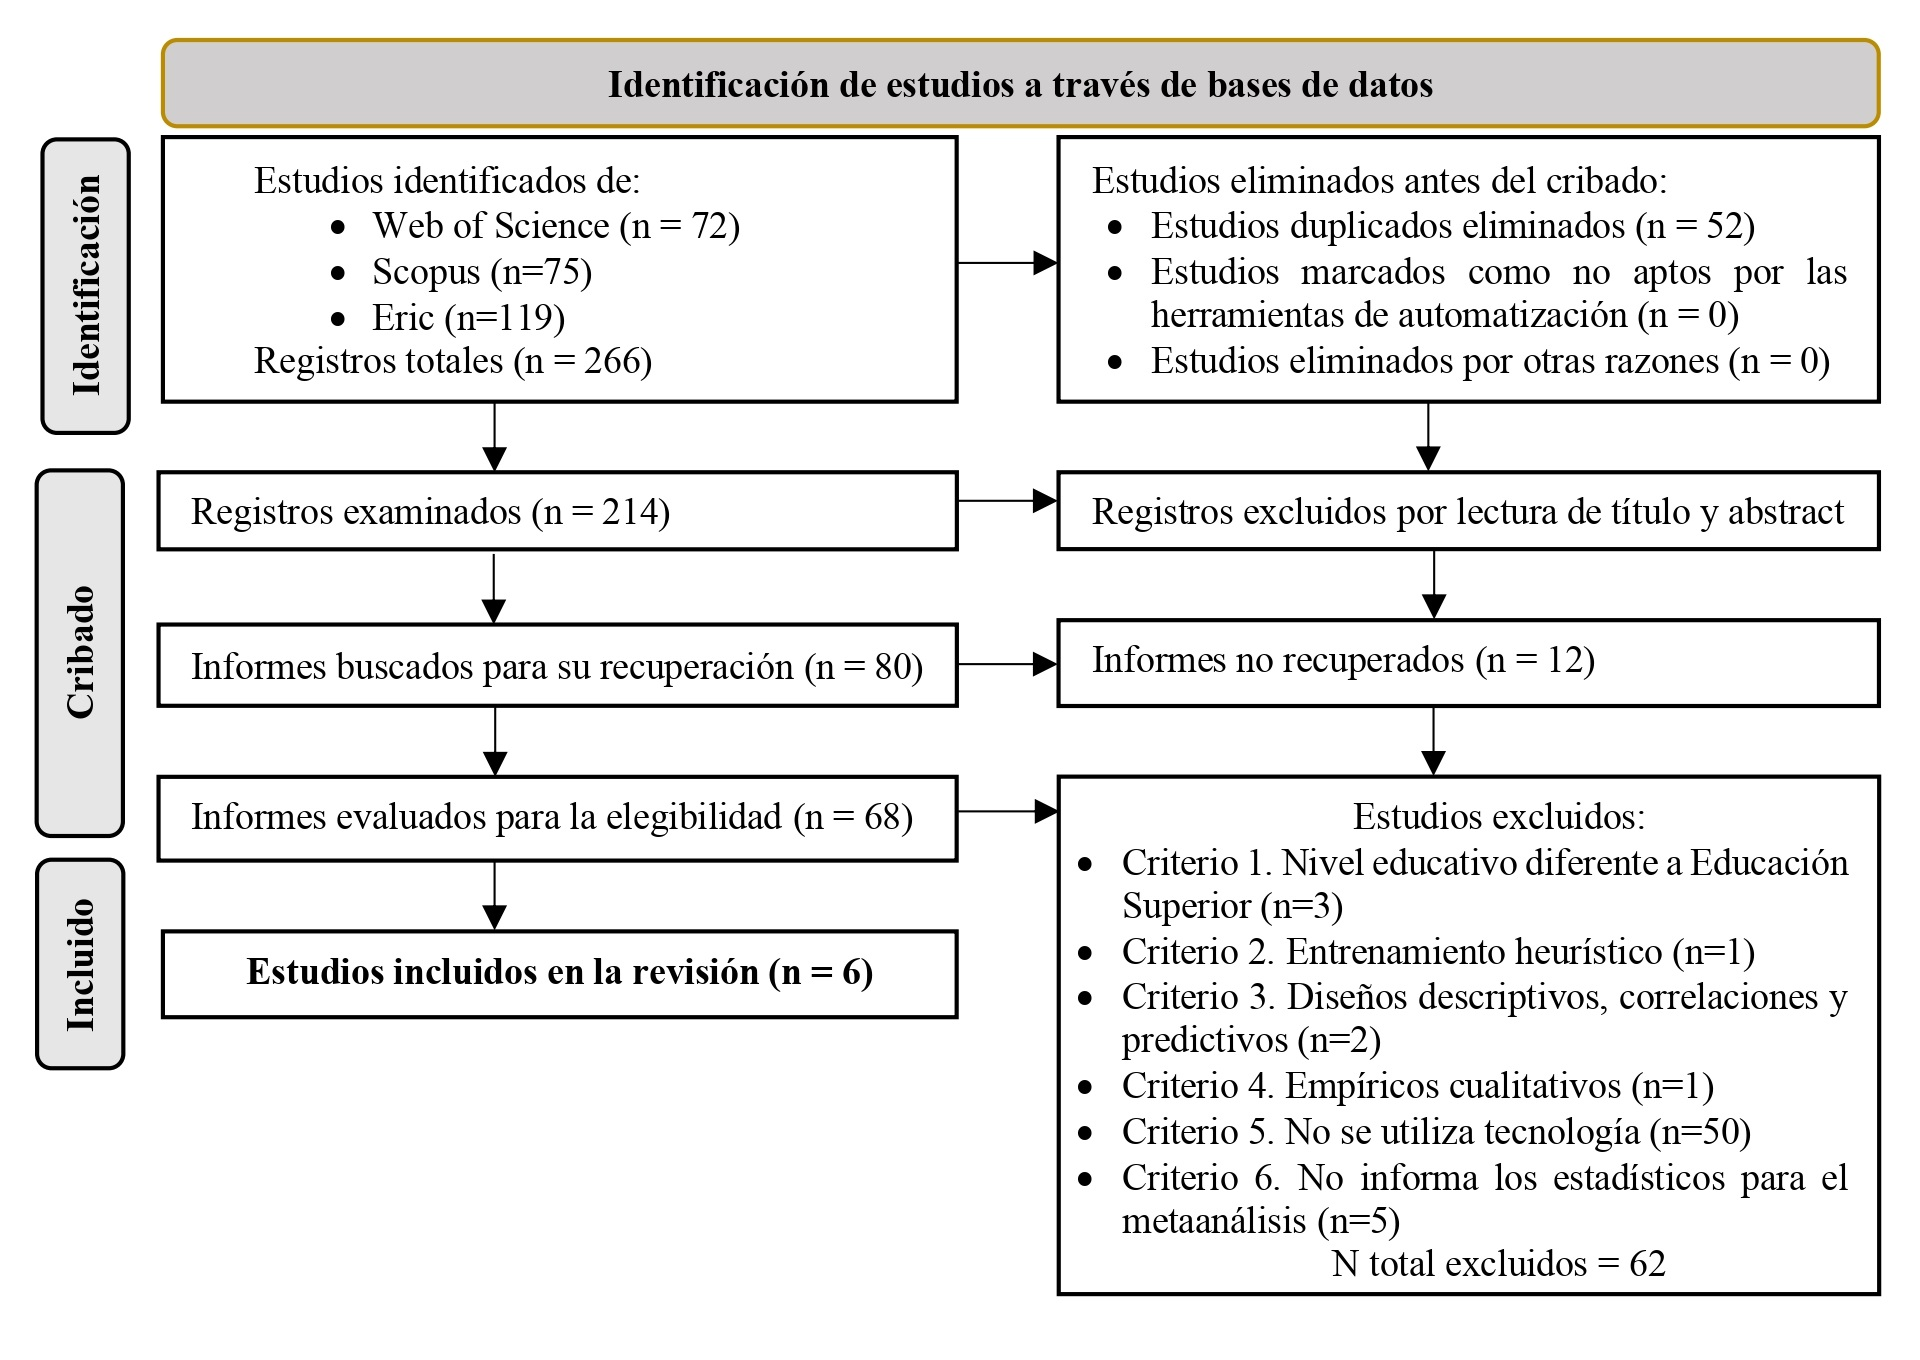
\includegraphics[width=\textwidth]{Fig1.jpeg}
 \caption{Flujograma}
 \label{fig1}
 \source{PRISMA, 2020}
\end{minipage}
\end{figure}


\subsection{Proceso de extracción de datos}

La extracción de la información fue realizada de forma independiente por el investigador principal y triangulada por el resto de los autores. Una primera parte incluyó una matriz para la extracción de datos sobre la caracterización de las intervenciones que incluyó la codificación de: nombre de la intervención, número, frecuencia, duración y contenido de cada sesión, modelos teóricos e instrumentos para la medición de la ARA, sustento teórico de tecnología, y recurso tecnológico utilizado (Material suplementario 2: \url{https://figshare.com/s/bf9885d580859f828a99}). Una segunda parte de extracción de datos fue para el metaanálisis que implicó la extracción de los estadísticos de tamaño muestral (\emph{n}), la media (\emph{M}), y la desviación estándar (\emph{DE}) para todas las medidas de resultado del grupo experimental, es decir el que participó de la intervención en los dos puntos temporales (pre y post test). 



\subsection{Análisis de datos}

La primera fuente de datos referido a la caracterización de los estudios fue analizada con estadística descriptiva de frecuencia. En el caso de la segunda fuente de datos estadísticos el análisis se realizó usando el software JAMOVI versión 2.3.21. El análisis se realizó utilizando la diferencia de medias estandarizada como medida de resultado dado que los estudios incluidos utilizaron diferentes instrumentos para medir la ARA. 

Dada la importancia que tiene la heterogeneidad estadística en la elección del modelo de metaanálisis, esta se midió mediante el estimador restringido de máxima verosimilitud ($\text{tau}^2$), la prueba Q de heterogeneidad y el índice $I^2$. Siempre que se detecta algún grado de heterogeneidad (es decir, $\text{tau}^2 > 0$, independientemente de los hallazgos de la prueba Q), se procede a proporcionar un intervalo de predicción para los resultados reales. Se consideró $I^2 \leq 50\%$ como punto de corte para la heterogeneidad aceptable, es decir, con valores por debajo de este punto se aplica un modelo de efectos fijos, mientras que con valores más altos ($I^2 >50\%$) se utilizó el modelo de efectos aleatorios, más conservador. 

Los residuos estudiados y las distancias de Cook se aplican para examinar si los estudios pueden ser atípicos y/o influyentes en el contexto del modelo. Los estudios con un residuo estudiado mayor que el percentil $100 \times (1 – 0.05/(2 \times 6))$ de una distribución normal estándar se consideran valores atípicos potenciales (es decir, utilizando una corrección de Bonferroni con alfa de dos caras $= 0.05$ para 6 estudios incluidos en el metaanálisis). Los estudios con una distancia de Cook mayor que la mediana más seis veces el rango intercuartílico de las distancias de Cook se consideran influyentes. 


\section{Resultados}

\subsection{Resultados sobre las características de las intervenciones}

Respecto de las características de las 6 intervenciones incluidas en esta investigación, solo una de estas usó un nombre para el programa que implementó, el cual se denominó “4Planning” \cite{lobos2021design}; en cuatro intervenciones se especifica el número de sesiones, siendo dos de estas de un total de 3 sesiones \cite{broadbent2020effects, van2020new}, una de 8 sesiones \cite{jansen2016fostering} y una de 9 sesiones \cite{lobos2021design}. La frecuencia de cada sesión se declaró en 2 estudios, en uno de ellos fue de 3 veces por semana \cite{bellhauser2016applying}, mientras que el otro la frecuencia fue de una vez a la semana \cite{van2020new}. En el caso de la duración de cada sesión, esta información se precisa en 4 estudios, siendo en tres de ellos de 90 minutos \cite{bellhauser2016applying, van2020new}, y en un estudio fue de 2 horas \cite{jansen2016fostering}. En relación con los contenidos trabajados en las intervenciones, en todos los casos incluyeron contenidos de las 3 fases del modelo de ARA, excepto en \textcite{lobos2021design}, en el cual no incorporaron contenidos de la fase de autoevaluación. 

El modelo de ARA de \textcite{zimmerman2000attaining} fue usado como base en todas las intervenciones. En relación con el sustento teórico tecnológico de las intervenciones, dos estudios lo declaran, en uno se usó el método de diseño centrado en el usuario \cite{lobos2021design}; y en otro estudio se usó la teoría cognitiva del aprendizaje multimedia \cite{mayer2003promise}. En el caso de los tipos de tecnologías incluidos en las intervenciones, en 3 estudios se utilizó LMS \cite{carrion2022effects,jansen2016fostering}, un estudio usó App \cite{lobos2021design} y en dos estudios se utilizó ambas tecnologías (LMS y Apps) \cite{bellhauser2016applying, broadbent2020effects}. 

El tamaño de la muestra de los estudios fluctuó entre n = 40 \cite{carrion2022effects} a $n = 473$ participantes \cite{lobos2021design}. Dos estudios se realizaron en Alemania \cite{bellhauser2016applying, van2020new}; dos estudios se realizaron en Taiwán \cite{carrion2022effects, jansen2016fostering}, un estudio fue realizado en Chile \cite{lobos2021design} y otro en Australia \cite{broadbent2020effects}. En todos los casos los instrumentos de ARA fueron escalas tipo Likert de autoinforme.


\subsection{Resultados del metaanálisis}

Se incluyeron en el análisis un total de $k = 6$ estudios. Las diferencias de medias estandarizadas observadas oscilaron entre 0.09 y 1.25, y todas las estimaciones fueron positivas (100\%). La diferencia de medias estandarizada, media estimada basada en el modelo de efectos aleatorios fue de 0.55 (IC del 95\%: 0.22, 0.88). Es decir, el resultado medio difería significativamente de cero demostrado en la prueba de tamaño del efecto total que fue significativa ($z = 3.25$, $p = 0.001$). 

Según la prueba Q, los resultados verdaderos parecen ser heterogéneos ($Q(5) = 25.98$, $p < 0.0001$, $\text{tau}^2 = 0.128$, $I^2 = 85.892\%$). Un intervalo de predicción del 95\% para los resultados reales viene dado por -0.315 a 1.260. Se observó una heterogeneidad alta ($I^2 = 85.67\%$), por lo que se deben interpretar los resultados cautelosamente, ya que indica que hay diferencias entre los estudios. Aunque se estima que el resultado medio es positivo, en algún estudio el resultado real puede ser negativo. Un examen de los residuos estudiados reveló que un estudio \cite{van2020new} tenía un valor superior a ± 2.638 y podría ser un valor atípico potencial en el contexto de este modelo. Pero, según las distancias de Cook, ninguno de los estudios puede considerarse excesivamente influyente. Ni la correlación de rangos ni la prueba de regresión indicaron asimetría alguna en el funnel plot ($p = 0.469$ y $p = 0.923$, respectivamente).

El peso estadístico de cada estudio analizado fue similar. Atendiendo a lo que se puede observar en el diagrama de bosque elaborado (forest plot), los resultados son favorables en la medición post intervención (ver \Cref{fig2}). Concretamente, en el forest plot se visualiza el símbolo de un diamante, el cual indica el resultado global de todos los estudios que se analizaron en este metaanálisis. Se observa que los 6 estudios otorgan un dictamen favorable a la post intervención y, por tanto, se puede señalar que aquellos que participaron de una intervención con uso de tecnologías para mejorar la ARA fue positiva. Todo lo señalado está respaldado, pues la realización del modelo estadístico obtuvo un valor \emph{p} significativo ($p <.001$).

\begin{figure}[htbp]
\centering
\begin{minipage}{\textwidth}
 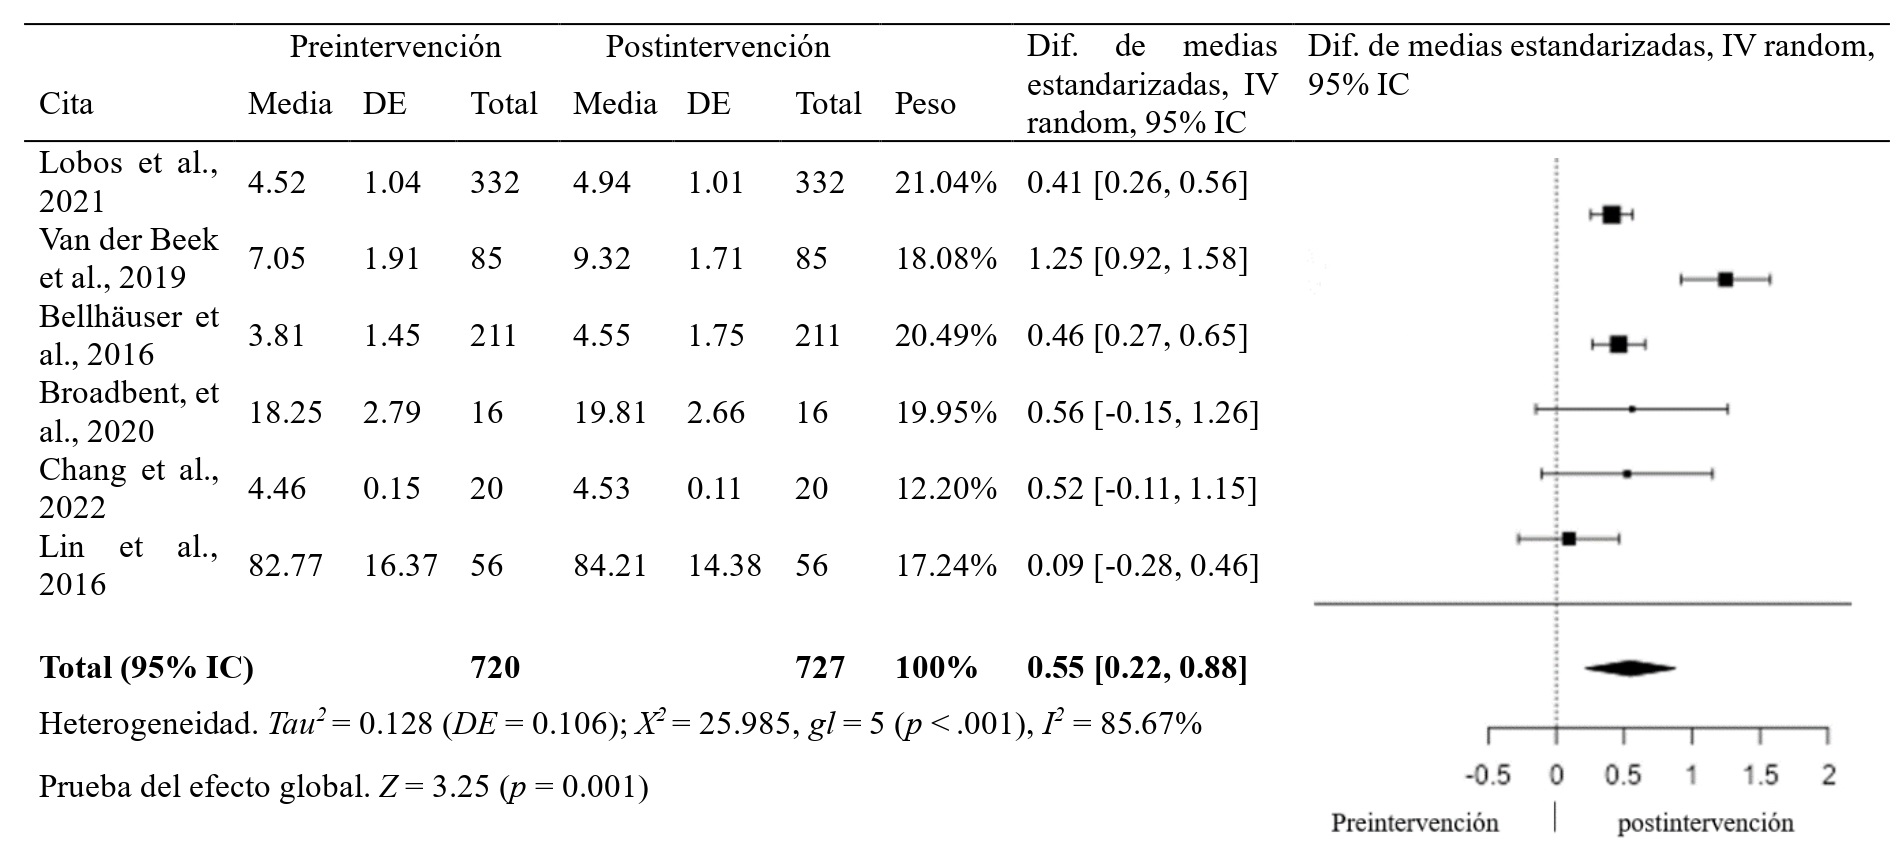
\includegraphics[width=\textwidth]{Fig2.jpeg}
 \caption{Diferencia de medias para variable autorregulación del aprendizaje}
 \label{fig2}
 \source{Elaboración propia.}
\end{minipage}
\end{figure}


\section{Discusión}

\subsection{Discusión de los resultados del objetivo 1. Caracterización de las intervenciones}

Este estudio se propuso como primer objetivo caracterizar las intervenciones para promover la ARA con uso de tecnología. Como resultado se puede evidenciar que en ninguno de los estudios se proporcionó información completa de las sesiones (número, frecuencia, duración). Este resultado es consistente con lo encontrado en investigaciones previas, por ejemplo, un estudio analizó 141 intervenciones donde el 40\% utilizaron términos vagos y generales al describir las intervenciones, en lugar de delinear sus componentes específicos incluso algunas se describieron de forma tan inadecuada que fueron denominadas "caja negra”, siendo las intervenciones educativas las de mayor falencia en sus detalles \cite{conn2012unpacking}. Otro estudio encontró que en la mayoría de las intervenciones vinculada a educación (59\%) faltaba información importante referida a la descripción del modo de realización de la intervención, número de sesiones, frecuencia de las sesiones y duración total \cite{palomares2012inadequate}. 

Por lo tanto, aunque los investigadores destacan la relevancia de detallar las intervenciones, desafortunadamente, la realidad es que estas se describen de forma incompleta e inconsistente. Proporcionar detalles suficientes sobre las intervenciones, son un aspecto fundamental del proceso científico pues: permite desarrollar una práctica basada en la evidencia; facilita su replicación e implementación en el entorno educativo; permite valorar la viabilidad y factibilidad de su implementación en un análisis coste-beneficio, puede evitar futuras pruebas innecesarias de intervenciones ineficaces; permiten comparar la eficacia entre distintos estudios mediante métodos metaanalíticos. Por el contrario, cuando la información es vaga, está poco detallada o falta por completo, dificulta la comprensión y evaluación crítica de los hallazgos y su contribución puede ser cuestionable \cite{stanley2018meta}. De hecho, un estudio analizó la replicabilidad de la investigación cuantitativa en educación tecnológica y en sus resultados los autores estimaron que al menos el 56\% de los estudios se replicarían, concluyendo en la necesidad de invertir esfuerzos en caracterizar las intervenciones minuciosamente para asegurar un alto valor en ser replicados como condición necesaria para garantizar un rigor continuo \cite{buckley2022estimating}.

En lo que respecta a los modelos teóricos de ARA, se pudo identificar que en todas las intervenciones (100\%) se consideró el modelo de \textcite{zimmerman2000attaining} proveniente de la teoría social cognitiva, lo que es consistente con lo encontrado en una revisión sistemática sobre ARA donde se pudo evidenciar la robusta influencia de esta teoría en la investigación referida a la autorregulación. Ahora bien, es importante tener en perspectiva otros modelos teóricos que permitan poner en contexto el ARA, por ejemplo, integrando la autorregulación, la corregulación y la regulación socialmente compartida del aprendizaje puesto que, si bien siempre se necesitan personas competentes capaces de regular su propio aprendizaje, la evolución de las exigencias de los estudiantes universitarios y futuros profesionales implica un cambio y tránsito desde el enfoque individual al colectivo. La colaboración y el trabajo en equipo es un escenario imprescindible para la solución de problemas educativos complejos donde la integración de procesos corregulados contribuye a las respuestas de profesionales de alta calidad en la nueva era de desafíos laborales e investigativos \cite{bransen2022putting}. 

Por otra parte, en lo que respecta a los modelos teóricos tecnológicos de las intervenciones, sOlo en 2 estudios (30\%) se describió algún componente. En la investigación de \textcite{lobos2021design}, se utilizó el "diseño centrado en el usuario" (DCU) que es un método reconocido en el diseño de aplicaciones web, el cual permite que los usuarios finales influyan en la forma en que se realiza un determinado diseño \cite{williams2009user}. Un ejemplo de productos que se logran a partir de un DCU son los Wireframes y Prototipos de las Apps. En la investigación de \textcite{van2020new}, se consideró la Teoría cognitiva del aprendizaje multimedia \cite{mayer2003promise}, la que estudia cómo los diseñadores deben estructurar un desarrollo multimedia y cómo aplicar estrategias cognitivas para ayudar al estudiantado a aprender de forma eficaz. Esta se basa en tres supuestos: canales duales, capacidad limitada y procesamiento activo. Los estudiantes aprenden utilizando diferentes recursos gráficos (esquemas, fotos, mapas, animaciones y/o vídeos) y texto impreso o hablado los que pueden combinarse o utilizarse por separado. Por tanto, aún es incipiente la incorporación de teorías provenientes de la tecnología educativa, en este sentido, se requiere que las intervenciones diseñadas para promover la ARA intencionen la consideración de fundamentos teóricos proveniente de tres áreas: 

\begin{enumerate}
    \item teorías de ARA
    \item teorías de tecnología educativa y
    \item teorías de enseñanza aprendizaje (ver \Cref{fig3}). 
\end{enumerate}

\begin{figure}[htbp]
\centering
\begin{minipage}{.5\textwidth}
 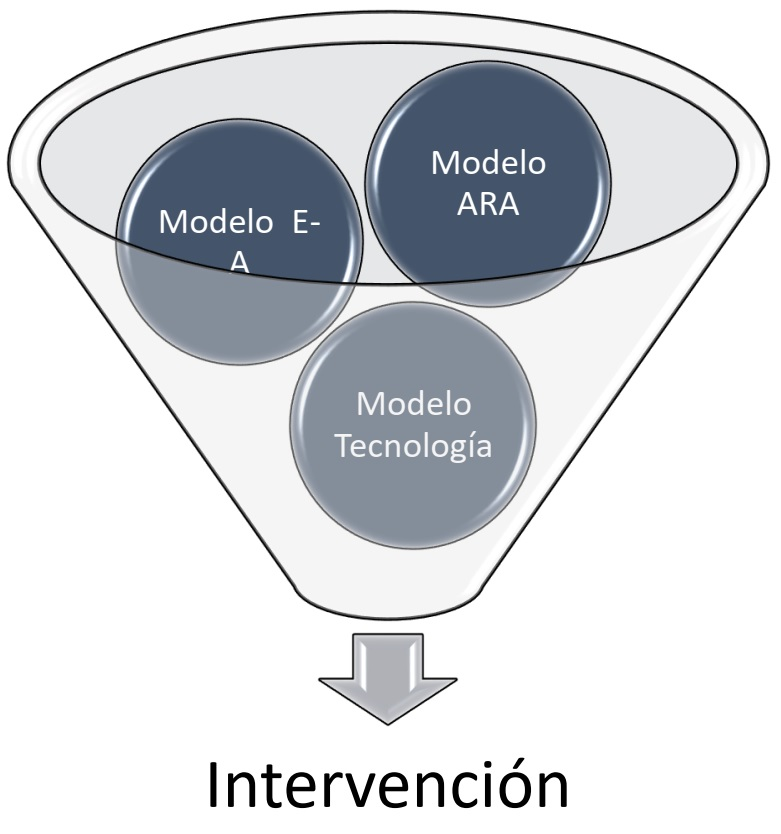
\includegraphics[width=\textwidth]{Fig3.jpeg}
 \caption{Componentes teóricos fundamentales en el diseño de intervenciones para la promoción de la ARA}
 \label{fig3}
 \source{Elaboración propia.}
\end{minipage}
\end{figure}

En cuanto a los recursos tecnológicos utilizados para implementar las intervenciones, estos fueron los LMS y Apps. Sin embargo, es necesario avanzar en la selección y especificación de diferentes recursos tecnológicos cuando se diseñan las intervenciones con el objetivo de promover la ARA. Actualmente se disponen de las denominadas Tecnologías Emergentes en la Educación (TEE), definidas como herramientas, tecnologías, innovaciones y avances utilizados en diversos contextos educativos para servir a diversos fines relacionados con la educación, caracterizado por cambiar rápidamente, por lo que siempre están evolucionando y tienen potencial para transformar las prácticas sociales \cite{neira2017emerging}. Algunos ejemplos de TEE son la realidad virtual, realidad aumentada, analítica de aprendizaje, inteligencia artificial, aprendizaje automático, internet de las cosas (IoT), computación en la nube, automatización, uso de las tecnologías 5G, aprendizaje basado en aplicaciones, clases magistrales digitales, big data, gamificación, 3D Printing, robótica, tecnología móvil etc. \cite{oliveira2019emerging}. 




\subsection{Discusión de los resultados del objetivo 2. Efectividad de las intervenciones}

 Actualmente, el metaanálisis es reconocido como un método valioso para la investigación específica del área de la educación \cite{bernardo2017meta}. Esta técnica permite sistematizar la evidencia cuantitativa acumulada ante un determinado objetivo investigativo caracterizado en su proceso por la precisión, la objetividad y la replicabilidad, permitiendo obtener como resultado la estimación combinada del tamaño del efecto y la evaluación de la heterogeneidad observada en un campo específico de la educación. Como consecuencia de los hallazgos de un metaanálisis, los investigadores pueden tomar decisiones y también formular nuevas hipótesis a partir de la evidencia \cite{moher2015preferred}. 

En particular, en este estudio y a partir de los resultados del metaanálisis es posible inferir que las intervenciones con uso de tecnología para la promoción de la ARA en universitarios logran un efecto positivo, es decir, los estudiantes incrementan sus procesos regulatorios. Este hallazgo es consistente con otros metaanálisis que han estudiado el efecto de intervenciones con uso de tecnologías para mejorar otras variables educativas. Por ejemplo, un estudio se propuso examinar, en qué medida el uso de la realidad aumentada (RA) mejoraba las experiencias de aprendizaje y sus resultados encontraron un efecto medio de la RA sobre la eficacia del aprendizaje ($d = .64$, $p < .001$) \cite{garzon2019systematic}. Otro estudio de metaanálisis se propuso integrar la investigación empírica cuantitativa sobre gamificación en entornos educativos y su impacto en los resultados de aprendizaje del estudiantado, donde sus hallazgos evidenciaron un TE global de $g = .464 [.244 a .684]$ a favor de la condición de ludificación, considerándose un tamaño del efecto de pequeño a mediano \cite{huang_impact_2020}.

En definitiva, es posible señalar que el resultado del presente metaanálisis es consistente con la integración de los hallazgos previos identificados en la literatura especializada, que han realizado otros estudios de metaanálisis sobre el efecto del uso de las tecnologías para mejorar variables psicoeducativas \cite{palomares2012inadequate, rojas2022analysis}. Por tanto, se confirma que los programas de intervención que incluyen tecnologías en contextos educativos obtienen resultados positivos en el proceso de enseñanza-aprendizaje y favorecen el desarrollo de habilidades transversales en el estudiantado, en este caso, específicamente en el incremento de la autorregulación del aprendizaje. Esto es particularmente relevante, dado que la investigación reciente, ha demostrado que durante la educación secundaria el estudiantado presenta trayectorias invariantes de autorregulación del aprendizaje y que estas trayectorias están en niveles subóptimos \cite{saez2023invariant}, consecuentemente identificar que intervenciones basadas en tecnologías muestran un efecto en incremento de los procesos autorregulatorios, resulta prometedor. 

\subsection{Limitaciones y futuras líneas de investigación}

Como todo estudio, este metaanálisis debe considerar algunas limitaciones para su interpretación cautelosa. Si bien fueron seleccionados los estudios que contaban con la información estadística suficiente para llevar a cabo la investigación, a nivel de descripción de las intervenciones, en todos los estudios faltaron elementos para su adecuada replicabilidad. Otra posible limitación, es que si bien en todos los estudios se utilizó un mismo tipo de instrumento para mediar la ARA (escalas tipo Likert de autoinforme), estos tienen aprensiones por parte de algunos investigadores, especialmente en lo referido a los procesos cognitivos involucrados en la respuesta a elementos de autoinforme bajo diversas condiciones de deseabilidad social (sesgos) \cite{holtgraves2004social}. También es importante considerar que la aplicación de un metaanálisis con un modelo de efectos aleatorios posibilita que los hallazgos obtenidos sean generalizables considerando muestras con características similares, por esto, la generalización debe hacerse con cautela y teniendo en cuenta que los estudios analizados fueron en estudiantes universitarios. Finalmente, los estudios seleccionados provienen de la búsqueda realizada en tres bases de datos y, por tanto, podrían existir otras experiencias de intervenciones en otras metabases. 

Futuras investigaciones podrían avanzar en el diseño de intervenciones con diferentes tecnologías emergentes para probar su efectividad en la promoción de estudiantes más autorregulados. También desplegar diferentes programas en otros niveles del sistema educativo, por ejemplo, en educación secundaria, de esta forma fomentar el desarrollo de habilidades autorregulatorias disposicionales, cognitivas y metacognitivas en etapas previas a la Educación Superior permitiría capacitar a los estudiantes con las habilidades necesarias que le permitan afrontar más fácilmente las exigencias de la etapa educativa. 


\section{Conclusiones}

A partir de la evidencia presentada en este metaanálisis se pueden delimitar varias conclusiones. Primero, las intervenciones para promover la ARA con uso de recursos tecnológicos evidencian un efecto significativo y positivo. Segundo, el detalle de las características de las intervenciones se describe de forma insuficiente. Se promueve la necesidad de que los investigadores detallen las intervenciones para su replicabilidad (numero, frecuencias, duración de las sesiones). Tercero, es importante que las intervenciones consideren en su diseño sólidos fundamentos teóricos, no solo explicitando su sustento en algún modelo de ARA, sino también en modelos teóricos de las tecnologías y modelos teóricos de enseñanza aprendizaje. Cuarto, en lo que respecta a los modelos teóricos de ARA, se pudo identificar que en todas las intervenciones se consideró el modelo de \textcite{zimmerman2000attaining}, pero se requiere intervenciones que en el sustento teórico considere otros modelos que permitan poner en contexto el ARA como por ejemplo las teorías de corregulación y la teoría de modelos de regulación socialmente compartida del aprendizaje, lo que contribuiría al cambio, transitando del enfoque individual al colectivo. Quinto, es relevante avanzar a la evaluación de la efectividad de intervenciones con uso de diferentes tecnologías emergentes propios de la nueva era que se han vinculado a resultados educativos exitosos. Sexto, se necesita la propuesta de nuevas intervenciones incrustadas en los curriculum e implicación de los docentes. Séptimo, requiere impulsar nuevos métodos de medición de la efectividad de las intervenciones para disminuir posibles sesgos propios de escalas de autoinforme, especialmente considerando que la ARA es una competencia y como tal, medir la habilidad autorreportada no da cuenta de su capacidad de ejecución en situaciones académicas específicas. Finalmente, se promueve el desarrollo de la ARA tempranamente en niveles educativos previos a la universidad, puesto que la ARA y sus variables integrantes, no es un rasgo sino más bien, habilidades entrenables que puestas en práctica permiten el logro de niveles adecuados de esta competencia. 

\section{Agradecimiento}
Al Proyecto FONDECYT de Iniciación en Investigación 2020 Nº11201054, titulado: “La relación recíproca entre la autorregulación del profesor y la autorregulación del aprendizaje y desempeño académico del estudiante. Un modelo explicativo en Educación Media”.

\printbibliography\label{sec-bib}
% if the text is not in Portuguese, it might be necessary to use the code below instead to print the correct ABNT abbreviations [s.n.], [s.l.]
%\begin{portuguese}
%\printbibliography[title={Bibliography}]
%\end{portuguese}


%full list: conceptualization,datacuration,formalanalysis,funding,investigation,methodology,projadm,resources,software,supervision,validation,visualization,writing,review
\begin{contributors}[sec-contributors]
\authorcontribution{Fabiola Sáez-Delgado}[conceptualization,datacuration,formalanalysis,methodology,supervision,validation,visualization,writing]
\authorcontribution{Francisca Parra}[conceptualization,writing]
\authorcontribution{Pilar Jara}[conceptualization,supervision,validation]
\authorcontribution{Javier Mella Norambuena}[conceptualization,datacuration,formalanalysis,software,writing]
\authorcontribution{Yaranay López Angulo}[validation,review]
\end{contributors}

\end{document}
